\documentclass[
	12pt,
	a4paper,
	BCOR10mm,
	%chapterprefix,
	DIV14,
	headsepline,
	%twoside,
	%openright
]{scrreprt}

\KOMAoptions{
	listof=totoc,
	bibliography=totoc,
	index=totoc
}

\usepackage[T1]{fontenc}
\usepackage[utf8]{inputenc}

\usepackage{lmodern}

\usepackage[ngerman,english]{babel}

\usepackage[toc]{appendix}
\usepackage{eurosym}
\usepackage{fancyhdr}
\usepackage{graphicx}
\usepackage[htt]{hyphenat}
\usepackage{listings}
\usepackage{microtype}
\usepackage[list=true,hypcap=true]{subcaption}
\usepackage{units}

\usepackage{varioref}
\usepackage[hidelinks]{hyperref}
\usepackage[capitalise,noabbrev]{cleveref}

\usepackage{wrapfig}
\usepackage{float}
\usepackage{amssymb,amsmath,amsthm,amsfonts}

\newtheorem{theorem}{Theorem}
\newtheorem{lemma}{Lemma}
\newtheorem{definition}{Definition}
\newtheorem{notation}{Notation}
%\newtheorem{proof}{Proof}

\usepackage{mathtools}
\DeclarePairedDelimiter{\ceil}{\lceil}{\rceil}
\DeclarePairedDelimiter{\floor}{\lfloor}{\rfloor}
\DeclarePairedDelimiter{\abs}{\lvert}{\rvert}

\renewcommand*{\thefootnote}{\fnsymbol{footnote}}

\lstset{
	basicstyle=\ttfamily,
	frame=single,
	numbers=left,
	language=C,
	breaklines=true,
	breakatwhitespace=true,
	postbreak=\hbox{$\hookrightarrow$ },
	showstringspaces=false,
	tabsize=4,
	captionpos=b,
	morekeywords={gboolean,gpointer,gconstpointer,gchar,guchar,gint,guint,gshort,gushort,glong,gulong,gint8,guint8,gint16,guint16,gint32,guint32,gint64,guint64,gfloat,gdouble,gsize,gssize,goffset,gintptr,guintptr,int8_t,uint8_t,int16_t,uint16_t,int32_t,uint32_t,int64_t,uint64_t,size_t,ssize_t,off_t,intptr_t,uintptr_t,mode_t}
}

\makeatletter
\renewcommand*{\lstlistlistingname}{List of Listings}
\makeatother

\begin{document}

\begin{titlepage}
	\begin{center}
		{\titlefont\huge SCIL - Scientific Compression Interface Library\par}

		\bigskip
		\bigskip

		{\Large Project Report\par}

		\bigskip
		\bigskip

		{\large Arbeitsbereich Wissenschaftliches Rechnen\\
		Fachbereich Informatik\\
		Fakultät für Mathematik, Informatik und Naturwissenschaften\\
		Universität Hamburg\par}
	\end{center}

	\vfill

	{\large\begin{tabular}{ll}
		Vorgelegt von:  & Armin Schaare \\
		E-Mail-Adresse: & \href{mailto:adresse@email.de}{3schaare@informatik.uni-hamburg.de} \\
		Matrikelnummer: & 6423624 \\
		Studiengang:    & Informatik \\
		\\
		Hamburg, den 05.04.2016
	\end{tabular}\par}
\end{titlepage}

\chapter*{Abstract}

\thispagestyle{empty}


SCIL is a compression library for the programming language C. It uses a
repertoire of conventional as well as specifically developed compression
methods. Which method it will choose depends on user provided parameters
including goal error tolerances and throughputs. Based on these information,
SCIL compressses the data lossy or lossless. \par
Benchmarking of SCIL in its current state has shown that some algorithms
in its repertoire never produce better results than others. Further including of
other algorithms, excelling at compressing data of specific characteristics, is
needed to make SCIL beneficial. \par
This project is still in early development with much of the core functionality
not yet implemented. Features which are still to be implemented are marked as
such throughout the report.

\tableofcontents

\chapter{Introduction}
\label{Introduction}

\section{Data Compression}

\bigskip

Data compression is the encoding of information to reduce its bit size while
still adequately representing the original information \cite{wiki:dc}.
Thus data compression can be used to maximize effective storage capacities of
given hardware as well as reducing the load on bandwidth limited networks.
Large amounts of data generated in scientific as well as commercial research
environments and limited budgets for data storage and processing give rise to
the need of better and faster compression techniques. The Large Hadron Collider
at CERN for example is generating 600 terabytes of collision event data per
second. Unable to process such volumes of data, scientists filter out the most
promising data, generally leaving 100 - 200 megabytes per second of 'interesting'
information which needs to be stored \cite{cern_data}. Another example where
data compression is very applicable is climate research. In particle collision
data not many interesting events are of concern, whereas for climate research it is
beneficial to record and process as much available data as possible
\cite{clim_data}. In any case, compression allows more data to be stored and
processed, contibuting to better and faster research.

\begin{wrapfigure}{l}{0.6\textwidth}
	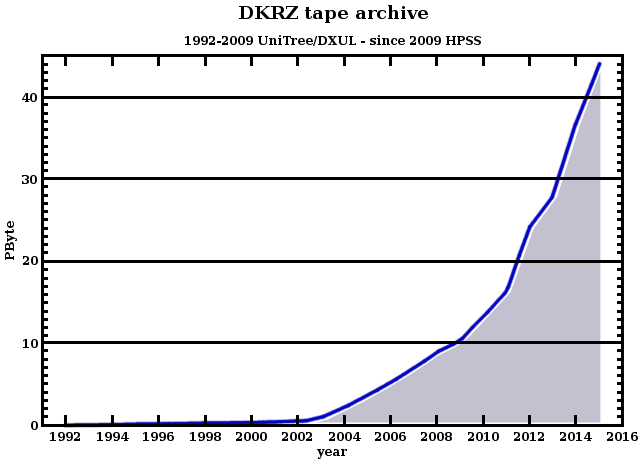
\includegraphics[width=0.9\linewidth]{DKRZ_data_growth.png}
	\caption{DKRZ data growth redrawn\\ \cite{data_graph}}
	\label{fig:dkrz}
\end{wrapfigure}

\cref{fig:dkrz} illustrates the increasing data usage at the German Climate
Computing Center in Hamburg (DKRZ). Until now data compression at the DKRZ
already has been put to practise but "storage capacity does not grow as fast as
computation power" \cite{strg_cap}. Therefore optimizations regarding data
reduction are an effective method to minimize the need of upscaling existing
data archives.

\clearpage

\section{SCIL}

To further exploit the potential of both lossy and lossless compression in
research, SCIL is being developed. SCIL is the Scientific Compression Interface
Library for the programming language C. Having not only conventional but also
specifically developed compression algorithms integrated, it is able to compress
data in a variety of ways. After calling the program
'scil-config'\footnote{Not yet implemented} to configure SCIL for the running
platform, each compression can be customized by providing parameters such as:

\bigskip

\begin{itemize}
	\item Absolute/Relative error tolerance
	\item Performance of compression in MB/s
	\item Dimensional layout of the data
\end{itemize}

\bigskip

Based on these parameters, the platform dependent configuration and the
characteristics of the data itself, SCIL will automatically choose the best
fitting compression algorithm at disposal\footnotemark[\value{footnote}].\par

\setcounter{footnote}{0}

\chapter{Design}
\label{Design}

\section{Problem Definition}

\bigskip

Many available compression algorithms perform different on distinct datasets.
Choosing the best algorithm for a given dataset is an assignment requiring
in depth knowledge of conventional compression methods. Furthermore it is
apparent that users are settling for one algorithm of their choice with which
they are compression various datasets. Algorithms performing better on some
datasets will be ignored compromising data reduction rates for consistency.\par
SCIL is a library which automates the task of algorithm choice while providing
a clean interface for compression and decompression. Its main goals are:

\bigskip

\begin{itemize}
	\item User-friendliness
	\item Data adaptability
	\item Extensibility
	\item Platform independence
\end{itemize}

\bigskip

\clearpage

\section{Design Description}

\bigskip

At the core of SCIL there are the two essential methods to compress and
decompress data, as well as a structure to hold the user specified compression
information. Calling the compression method invokes SCIL's internal workflow in
which it chooses the best compression methods out of available algorithms.
The decision on which algorithm to choose is not only based on the users
parameter input but also on the data characteristics and the platform specific
configuration of SCIL. After writing the compressed buffer it is possible to
decompress again by simply calling the decompression method of SCIL.
In the following subsections a more detailed explanation of SCILs workflow
will be presented.

\bigskip

\subsection{Algorithm Decision}

\bigskip

After validating the parameters of the compress function call, it is determined
if the user explicitly forced to compress with a certain algorithm. In that case
the compression commences, providing relevant user specified parameters to the
chosen method. Otherwise the compression parameters are checked to determine
whether a lossless compression is needed (if the user provided no parameters on
error tolerance) or if a lossy compression method suffices the users needs. In
case of lossless compression the parameter restricting compression speed is
the only one consulted\footnote{Not yet implemented}. If none is given, SCIL
will default to best compression rates, regardless of compression speed. If the
user provided arguments describing error tolerance, SCIL considers lossy
algorithms, optionally with a subsequent lossless
compression\footnotemark[\value{footnote}]. In either case the platform specific
configuration of SCIL [see subsec ...] and current data characteristics are of
interest. Analyzing the data for its characteristics is an optional
feature\footnotemark[\value{footnote}] as it can be very time-consuming - yet it
enables further customization of the compression by the user.

\setcounter{footnote}{0}

\clearpage

\subsection{Header Writing}

\bigskip

\renewcommand*{\thefootnote}{\arabic{footnote}}

The intermediate step between algorithm choice and actual compression is the
writing of meta data to the beginning of the compressed data buffer. This meta
data is often called header. The first byte in the header represents the
algorithm ID. Based on this number, SCIL is able to identify the correct decompression
method later on. The ID is the only part of the header guaranteed to be present.
Afterwards the data's dimensional layout will be written if the user chooses to
do so. Generally users are aware of the dimensional configuration of their data,
thus SCIL defaults to not storing it in the header\footnote{Currently always stores the dimensional configuration of the data}.
Nevertheless, storing the
dimensional layout in the header can be beneficial, for example if the data is
shared between users. At last, algorithm specific meta data is written. This
data is different from algorithm to algorithm and will be discussed in detail
in \cref{comp_data}.

\bigskip

\subsection{Compressing Data}
\label{comp_data}

\bigskip

Finally, the actual compression of the data commences. Depending on the chosen
algorithm, compression rates and speeds can vary widely. Current Compression
Algorithms at disposal include:

\bigskip

\begin{itemize}
	\item memcpy \footnote{As the trivial compression for benchmarking puposes}
	\item abstol
	\item gzip
	\item sigbits
	\item fpzip
	\item zfp, absolute tolerance
\end{itemize}

\setcounter{footnote}{0}

\bigskip

The abstol and sigbits algorithms are specifically developed for SCIL. A
detailed description of their functionality can be found in \cref{abstol} and
\cref{sigbits} respectively. All other compression methods are included from
independent projects. A reference to those projects can be found in the
bibliography of this report.

\clearpage

\subsection{Decompressing Data}

\bigskip

The decompression of data is invoked by calling the designated function. Since
compression relevant data has been stored in the header of the compressed
buffer, the user does not need to provide further information for decompression.
Defining a structure to hold dimensional data, however, is optional. If the user
decided to store the data's dimensional configuration at compression, this
provided structure will hold the dimensional configuration after decompression.
If no dimensional configuration has been stored in the header of the compressed
data, the number of dimensions in the provided structure will be set to
zero\footnote{Not yet implemented}.

\setcounter{footnote}{0}

\chapter{Example Code}

%In the following sections, example code is presented to illustrate the usage
%of SCIL. The example code is written in the programming language C and not in
%pseudo-code, due to SCIL currently being a pure C library.

\section{Compressing}

\bigskip

\begin{lstlisting}[caption=Compression with SCIL, label={lst:comp}]
// Providing user specified compression parameters
scil_hints hints;
hints.absolute_tolerance = 0.005;
hints.relative_tolerance_percent = 1.0;
hints.significant_bits = 5;
...

// Creating compression context
scil_context* context;
scilPr_create_context(&context, &hints);

// Writing dimensional layout (1D, 100 elements)
size_t* lengths = (size_t*)malloc(sizeof(size_t));
lenghts[0] = 100;
scil_dims_t dimensions = scil_init_dims(1, lengths);

// Allocating destination and source buffer
double* source = (double*)malloc(100 * sizeof(double));
byte* destination = (byte*)malloc(100 * sizeof(double) + SCIL_BLOCK_HEADER_MAX_SIZE);

// Write data to source buffer
...

// Variable holding compressed buffer size after compression
size_t compressed_size;

// Compress data
scil_compress(SCIL_DOUBLE, destination, &compressed_size, source, dimensions, context);
\end{lstlisting}

\clearpage

\section{Decompressing}

\bigskip

\begin{lstlisting}[caption=Decompression with SCIL, label={lst:decomp}]

// Providing size of compressed buffer
size_t source_size = ... ;

// Providing structure for dimensional configuration
size_t* lengths = (size_t*)malloc(sizeof(size_t));
scil_dims_t dimensions = scil_init_dims(1, lengths);

// How many values are compressed in the source buffer
size_t element_count = 100;

// Allocating destination buffer
double* destination = (double*)malloc(element_count * sizeof(double));

// Decompressing
scil_decompress(SCIL_DOUBLE, destination, dimensions, source, source_size);
\end{lstlisting}

\chapter{Conclusion}
\label{Conclusion}

\section{Benchmarking}

The data used for benchmarking was generated by 'mode 11' of Nathanael Huebbe's
C program for data generation. The bias parameter for all dataset was 0, the
discountFractor was equal the randomness of the data, as specified by this
report.

\subsection{Lossy Compression}

\bigskip

The following figures show the compression rates of different algorithms,
distinguishing between absolute and relative error tolerance. Each figure shows
the performances of the four chosen algorithms on a given dataset. The datasets
are different from each other in their randomness. Figure captions are
referencing to a visualization of the compressed data.

\begin{figure}[H]
	\centering
	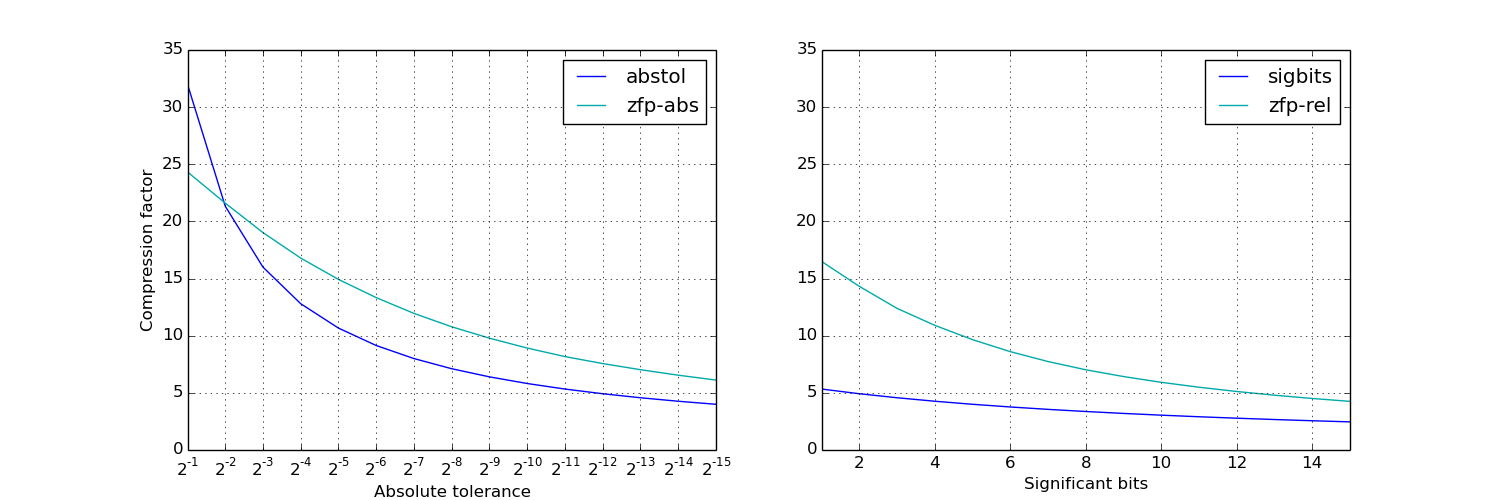
\includegraphics[width=\textwidth]{000_lossy_rates.png}
	\caption{Randomness 0.00, data \ref{000}}
	\label{fig:000_rate}
\end{figure}

\begin{figure}[H]
	\centering
	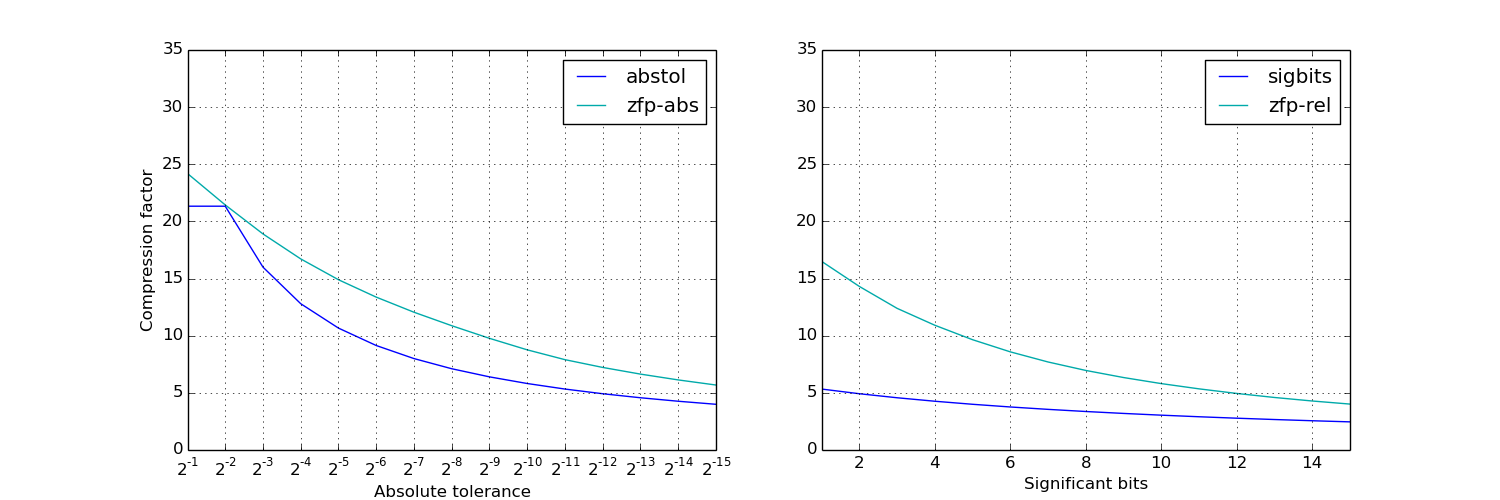
\includegraphics[width=\textwidth]{025_lossy_rates.png}
	\caption{Randomness 0.25, data \ref{025}}
	\label{fig:025_rate}
\end{figure}

\begin{figure}[H]
	\centering
	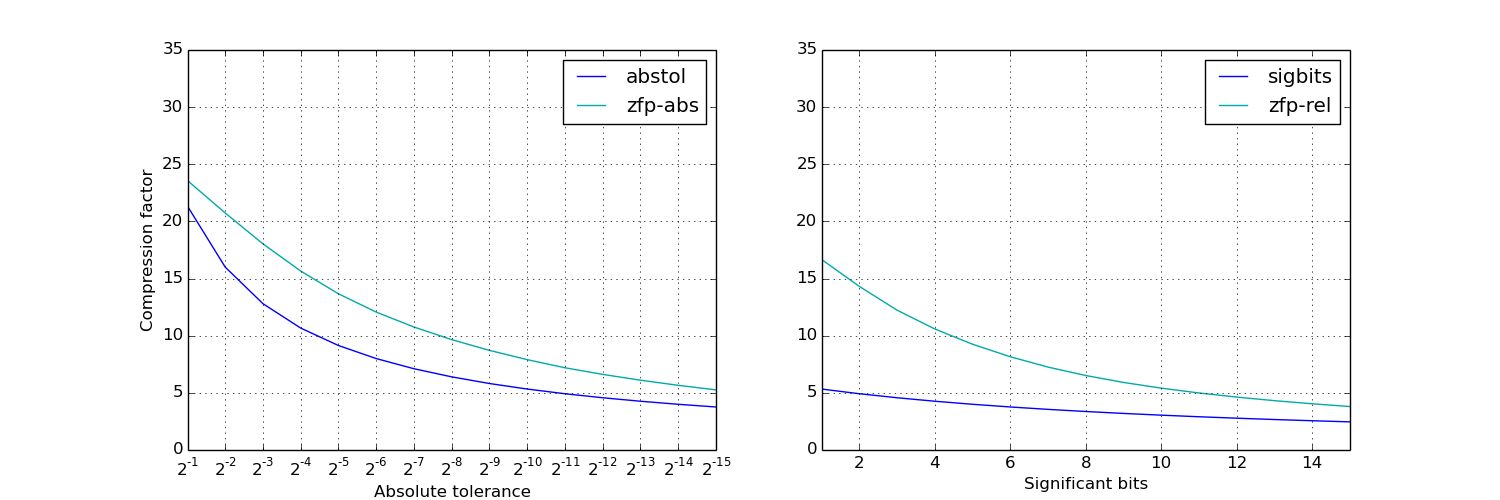
\includegraphics[width=\textwidth]{050_lossy_rates.png}
	\caption{Randomness 0.50, data \ref{050}}
	\label{fig:050_rate}
\end{figure}

\begin{figure}[H]
	\centering
	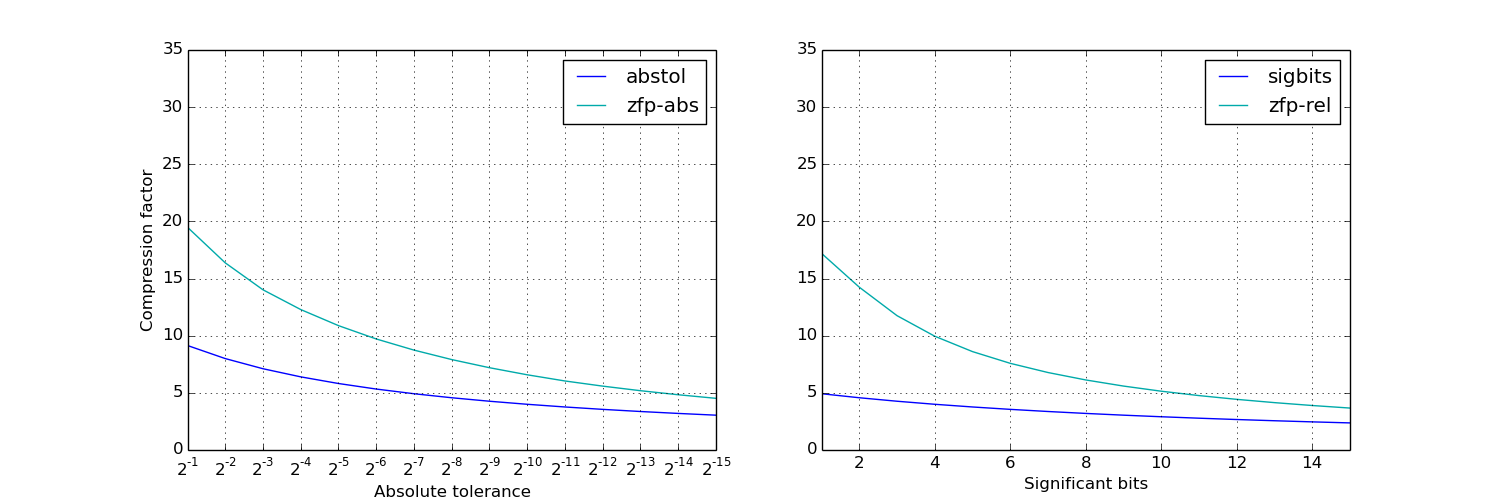
\includegraphics[width=\textwidth]{075_lossy_rates.png}
	\caption{Randomness 0.75, data \ref{075}}
	\label{fig:075_rate}
\end{figure}

\begin{figure}[H]
	\centering
	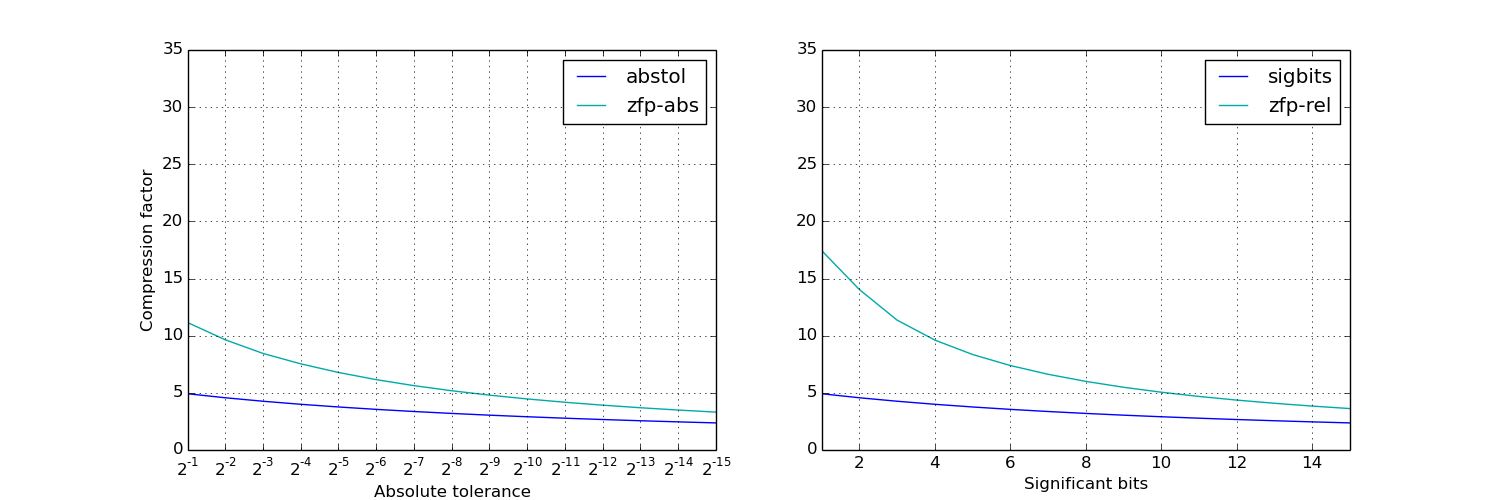
\includegraphics[width=\textwidth]{100_lossy_rates.png}
	\caption{Randomness 1.00, data \ref{100}}
	\label{fig:100_rate}
\end{figure}

\clearpage

\subsection{Lossless Compression}

\bigskip

This figure shows the compression rate of the chosen lossless methods.
Because an error tolerance in lossless compression is of no concern, only one
figure holds the information of all different data. The x-axis denotes the
randomness of the data.

\begin{figure}[H]
	\centering
	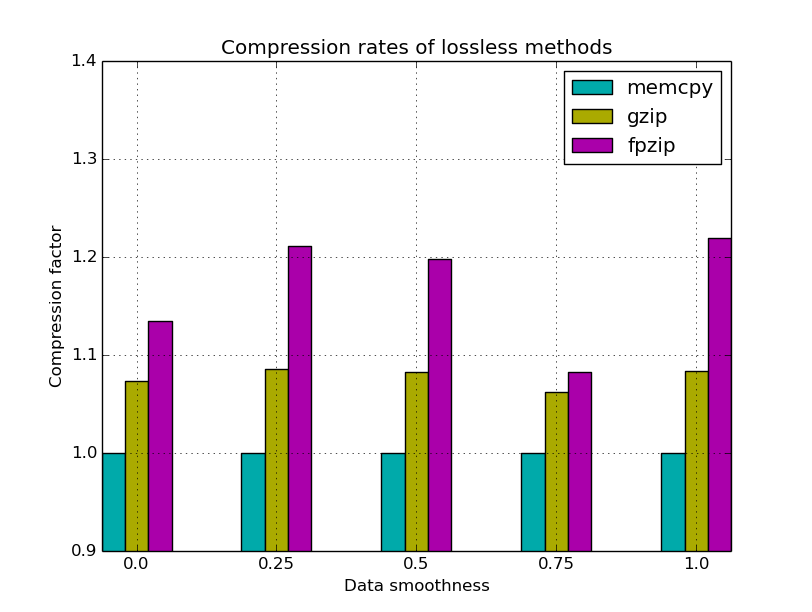
\includegraphics[width=0.6\textwidth]{c_rates_lossless.png}
	\caption{}
	\label{fig:lossless_rates}
\end{figure}

\subsection{Lossy and Lossless Throughput}

\bigskip

The performances of all currently implemented algorithms regarding throughput
can be seen in \ref{fig:through}.

\begin{figure}[H]
	\centering
	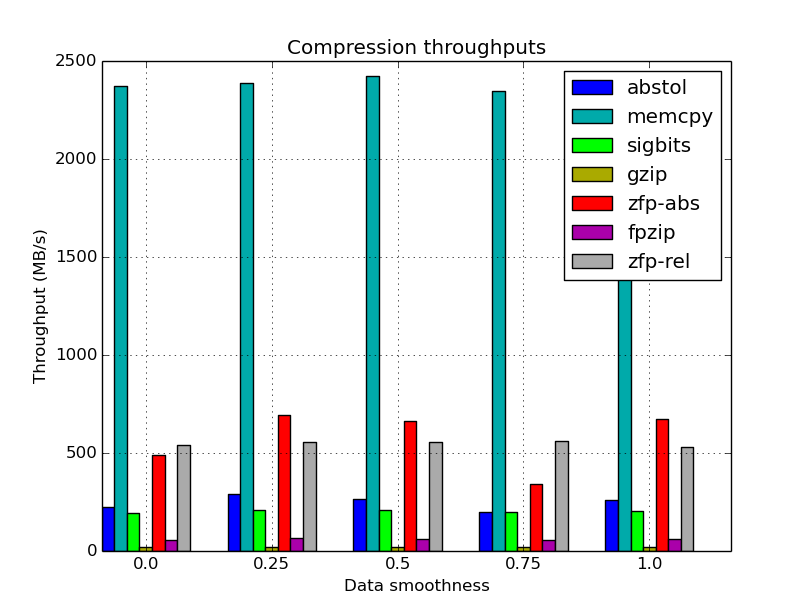
\includegraphics[width=0.6\textwidth]{throughputs.png}
	\caption{}
	\label{fig:through}
\end{figure}

\clearpage

\section{Evaluation}

\bigskip

With the current pool of algorithms, zfp should be the preferred algorithm
almost all of the time when compression lossy. The abstol and sigbits algorithms
do generally not reach compression rates of zfp, except with the most
specific and unrealistic data. Even the compression throughput is generally at
least two times better comparing zfp to abstol or sigbits. To be beneficial to
SCIL, abstol and sigbits have to be further optimized regarding compression
rates and speed. \par
Discussing lossless methods, fpzip is currently the best choice. gzip's
compression performance only came close to that of fpzip with data \ref{075}.
The throughput of fpzip is also better than that of gzip in all of the tested
data sets. \par
Those tests show, that the algorithm repertoire of SCIL is nowhere near ideal.
More compression methos shoud to be included, with each one performing differently
on different data, so that an automated algorithm choice would be beneficial.
In its current state, SCIL would always resort to using zfp for lossy or fpzip for
lossless compression, not exploiting its full potential by far.


\bibliographystyle{alpha}
\bibliography{literatur}

\appendix
\appendixpage

\chapter{abstol}
\label{abstol}

\bigskip

The abstol compression method works by projecting uncompressed values to their
nearest representating value, based on the user-provided absolute error
tolerance. After determining the minimum and maximum values of the data, abstol
calculates how many bits are needed to represent all numbers in the
minimum-maximum-range, given the absolute error tolerance. The headers of
abstol-compressed data buffers contain the minimum value found in the data, the
absolute tolerance and the bit size of compressed values. While compressing the
data, abstol packs the buffer tightly as described in \cref{bit_perf}.

\bigskip

\begin{definition} \label{D:abstol_nbits}
	Let $V_{min}$ be the minimum value in the data, $V_{max}$ the maximum value
	in the data, $\Delta{e} > 0$ the user provided absolute error tolerance and
	$N_{bit}$ the number of bits needed to represent a compressed value. For
	$\Delta{e}>0$, $N_{bit}$ can then be calculated as follows:
	\[
		N_{bit} =
			\ceil[\big]{
				\log_2{
					\left(
						1 + \frac{V_{max} - V_{min}}{2 * \Delta{e}}
					\right)
				}
			}
	\]
\end{definition}

\bigskip

\begin{definition} \label{D:abstol_enc}
	Let $E:\mathbb{R}\rightarrow\mathbb{N}$ be the function to encode values to
	their compressed representation and $R$ the round to nearest integer
	function. For $\Delta{e}>0$, $E$ is defined as follows:
	\[
		E\left(x\right) =
			R
				\left(
					\frac{x - V_{min}}{2 * \Delta{e}}
				\right)
	\]
\end{definition}

\bigskip

\begin{definition} \label{D:abstol_dec}
	Let $D:\mathbb{N}\rightarrow\mathbb{R}$ be the function to decode values to
	their compressed representation. For $\Delta{e}>0$, $D$ is defined as
	follows:
	\[
		D\left(x\right) = V_{min} + x * 2 * \Delta{e}
	\]
\end{definition}

\clearpage

\begin{theorem} \label{T:abstol}
	Let $V_i$ be the original value. For all $V_i \ge V_{min}$,
	$V_i \le V_{max}$ and $\Delta{e} > 0$, the absolute error of a value after
	a compression-decompression-cycle using the abstol algorithm is smaller or
	equal $\Delta{e}$.
\end{theorem}

\begin{proof}
	\begingroup
	\addtolength{\jot}{1em}
	\begin{align*}
	  \lvert D\left(E\left(V_i\right)\right) - V_i\rvert
	  &\stackrel{\ref{D:abstol_enc}\ref{D:abstol_dec}}{=}\abs[\big]{V_{min} + R\left(\frac{V_i - V_{min}}{2\Delta{e}}\right) * 2\Delta{e} - V_i} \\
	  &=\abs[\big]{V_{min} + \floor[\Big]{\frac{V_i - V_{min}}{2\Delta{e}} + 0.5} * 2\Delta{e} - V_i} \\
	  &\le\abs[\big]{V_{min} + \left(\frac{V_i - V_{min}}{2\Delta{e}} + 0.5\right) * 2\Delta{e} - V_i} \\
	  &=\abs[\big]{V_{min} + \left(V_i - V_{min}\right) + \Delta{e} - V_i} \\
	  &=\abs{\Delta{e}} \\
	  &=\Delta{e} \qedhere
	\end{align*}
	\endgroup
\end{proof}

\chapter{sigbits}
\label{sigbits}

\bigskip

The sigbits compression algorithm uses the provided relative error tolerance.
The relative error tolerance currently can be provided by three different
metrics. Percentage, Significant decimal places and significant bits (in the
mantissa). These metrics are converted into each other at the compression
context creation, upholding the most restrictive value. At this point only the
significant bits information is of relevance to the sigbits algorithm. \par
For the sigbits compression with relative error tolerance, it is crucial to
separate floating point values by sign, exponent and mantissa. After scanning
for the minimum and maximum signs as well as exponents in the data, sigbits calculates
how many bits are needed to represent all occurring signs and exponents in the
data. The provided significant bits information determines how many bits in the
mantissa are kept. Adding those three values together, the overall bit count of
one compressed number is determined.\par
The algorithm then commences to write the header. Stored information include

\begin{itemize}
	\item a sign id, specifying whether all values are positive, negative or if the data
			contains negative and positive numbers
	\item how many bits each values exponent requires
	\item how many bits each values mantissa requires
	\item the minimum exponent
\end{itemize}

After writing the header, the actual compression begins, packing compressed
values tightly as seen in \cref{bit_perf}.

\clearpage

\begin{definition} \label{D:sigbits_sdec}
	Let $S_{dec}$ be the number of significant decimal places and $S_{bit}$
	the number of significant bits. $S_{bit}$ can then be calculated as follows:
	\[
		S_{bit}=\ceil{S_{dec} * \log_{2}{10}}
	\]
\end{definition}

\bigskip

\begin{definition} \label{D:sigbits_rtol}
	Let $\rho_{e}$ be the relative error tolerance in percent and $S_{bit}$
	the number of significant bits. For $\rho_{e} > 0$ and $\rho_{e} \le 100$,
	$S_{bit}$ can then be calculated as follows:
	\[
		S_{bit}=\ceil[\Big]{
			log_2{
				\left(
					\frac{100}{\rho_{e}}
				\right)
			}
		}
	\]
\end{definition}

\bigskip

\begin{notation} \label{N:sigbits}
	As the signs and exponents of each value are just minimized and stored
	losslessly, the relative error happening at the compression is inherent to the
	mantissa. Therefore it suffices to prove that the mantissas value resides in
	the tolerated error margin.
\end{notation}

\bigskip

\begin{lemma} \label{L:sigbits}
	Let $m$ be the original mantissa, $m_c$ the mantissa after a
	compression-desompression-cycle of the sigbits algorithm and $S_{bit}$ the
	number of significant bits. The sigbits algorithm effectively replaces each
	binary digit bit with zero, upkeeping only the first $S_{bit}$ bits.
	Therefore following inequality holds:
	\[
		m_c > m - 2^{-S_{bit}}
	\]
\end{lemma}

\clearpage

\begin{theorem} \label{T:sigbits}
	Let $m$ be the original mantissa, $m_c$ the mantissa after a
	compression-desompression-cycle of the sigbits algorithm, $S_{bit}$ the
	number of significant bits and $\rho_e$ the relative error tolerance in
	percent. The relative error of the values mantissa after a
	compression-decompression-cycle of the sigbits algorithm is smaller than
	the provided relative error margin for $m\ge 1$ and $m_c\ge 1$.
\end{theorem}

\begin{proof}
	\begingroup
	\addtolength{\jot}{1em}
	\begin{align*}
		1 - \frac{m_c}{m}
		&\stackrel{\ref{L:sigbits}}{\le}1 - \frac{m-2^{-S_{bit}}}{m} \\
	  	&=\frac{2^{-S_{bit}}}{m} \\
		&=\frac{1}{m * 2^{S_{bit}}} \\
	  	&\stackrel{\ref{D:sigbits_rtol}}{=}\frac{1}{m * 2^{
				\ceil{
					\log_2{\frac{100}{\rho_{e}}}
				}
			}} \\
	  	&\le \frac{1}{m * 2^{
				\log_2{\frac{100}{\rho_{e}}}
			}} \\
	  	&=\frac{1}{m * \frac{100}{\rho_{e}}} \\
		&=\frac{\rho_e}{100 * m} \\
	  	&\le \frac{\rho_e}{100} \qedhere
	\end{align*}
	\endgroup
\end{proof}

\chapter{Bit Perfect Packing of Data}
\label{bit_perf}

\bigskip

Compressing buffers with the abstol or sigbits algorithm often leads to
compressed values not taking up multiples of eight bits space. Storing such
values bytewise would waste compression potential as there would be lots of
bits unused by the buffer. Packing values tightly together so that every bit
is written is a more reasonable approach. \par
The bit perfect writing of compressed data happens in the compression loop,
right after values are encoded. First the indices of the starting and ending
bytes are determined between which the value is written. If they are the same, the
value will be written entirely into the current byte, only being potentially
shifted to accomodate already written bits. Else the value spans multiple
bytes needing to be segmented via the help of bitmasks. With the segmentation
and bit-shifting of parts of the value it can be stored densely inside the
buffer. After all values have been written the compression concludes. \par
Reading compressed values for buffers using bit perfect packing is very
similar to writing. The decompression works by having an iterator variable in
the decompression loop, being incremented by the bit size of a compressed value.
Thus when dividing by eight it points to the current byte. The modulo with
eigth indicates the starting bit of the compressed value inside the current
byte. After determining start and end byte again, the value is being read and
shifted accordingly. In the case of a multiple byte spanning value, the separate
parts are read and shifted, using a bitwise and-operator to reconstruct the
original value.

\chapter{Data Visualization}

\bigskip

\begin{figure}[H]
  \centering
  \begin{minipage}[b]{0.49\textwidth}
    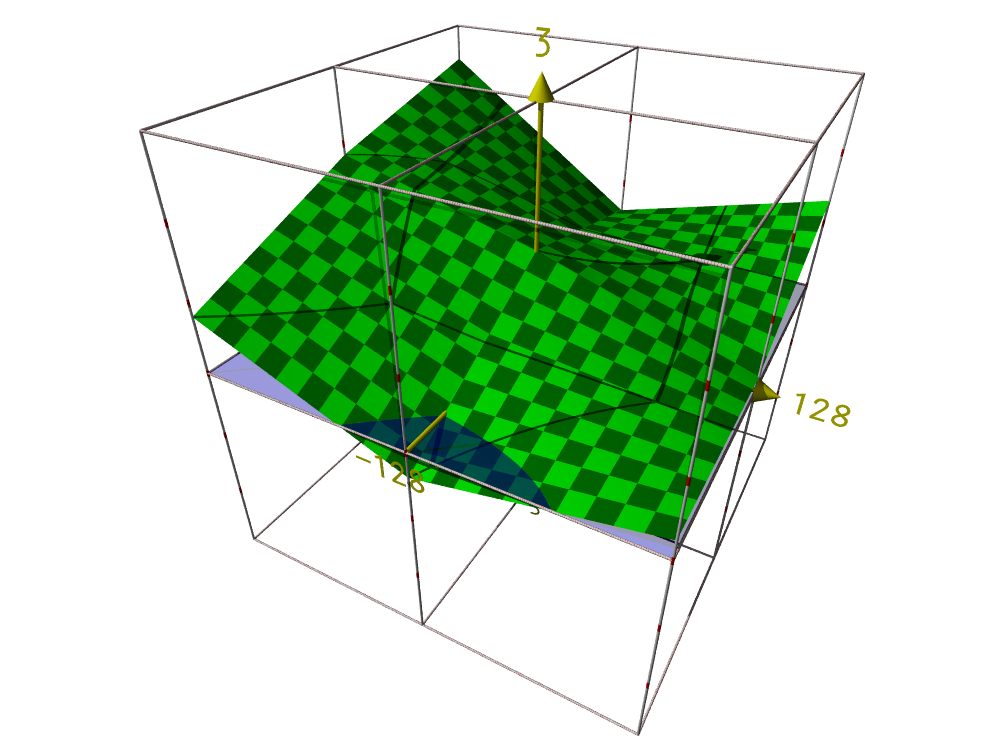
\includegraphics[width=\textwidth]{000.png}
    \caption{Randomness 0.00}
	\label{000}
  \end{minipage}
  \hfill
  \begin{minipage}[b]{0.49\textwidth}
    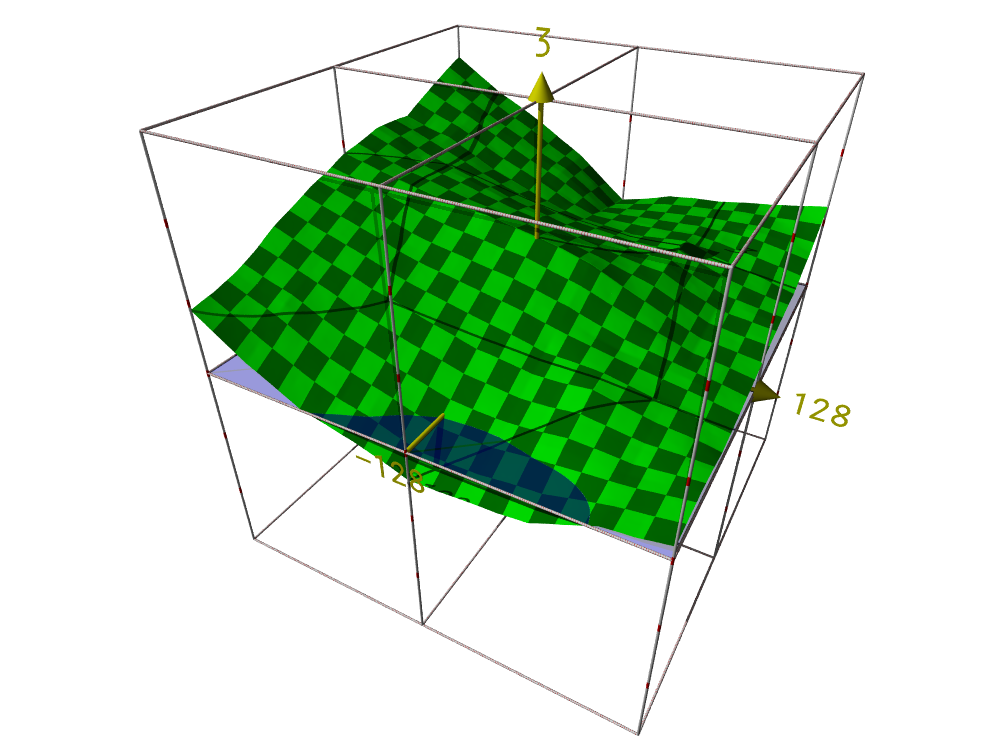
\includegraphics[width=\textwidth]{025.png}
    \caption{Randomness 0.25}
	\label{025}
  \end{minipage}
\end{figure}

\begin{figure}[H]
  \centering
  \begin{minipage}[b]{0.49\textwidth}
    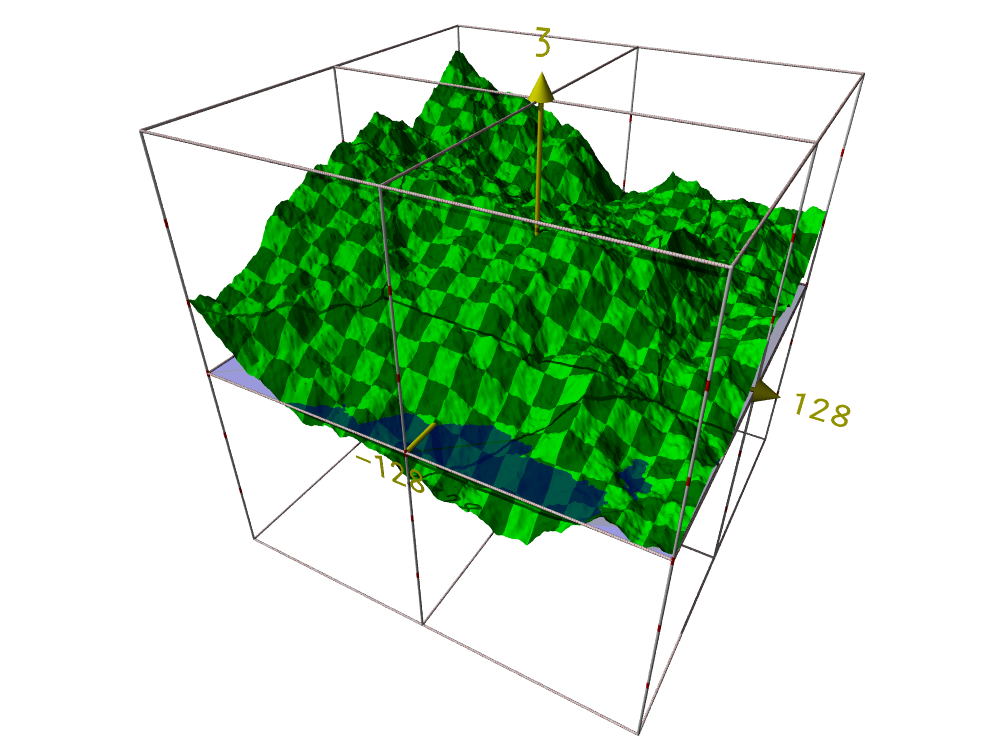
\includegraphics[width=\textwidth]{050.png}
    \caption{Randomness 0.50}
	\label{050}
  \end{minipage}
  \hfill
  \begin{minipage}[b]{0.49\textwidth}
    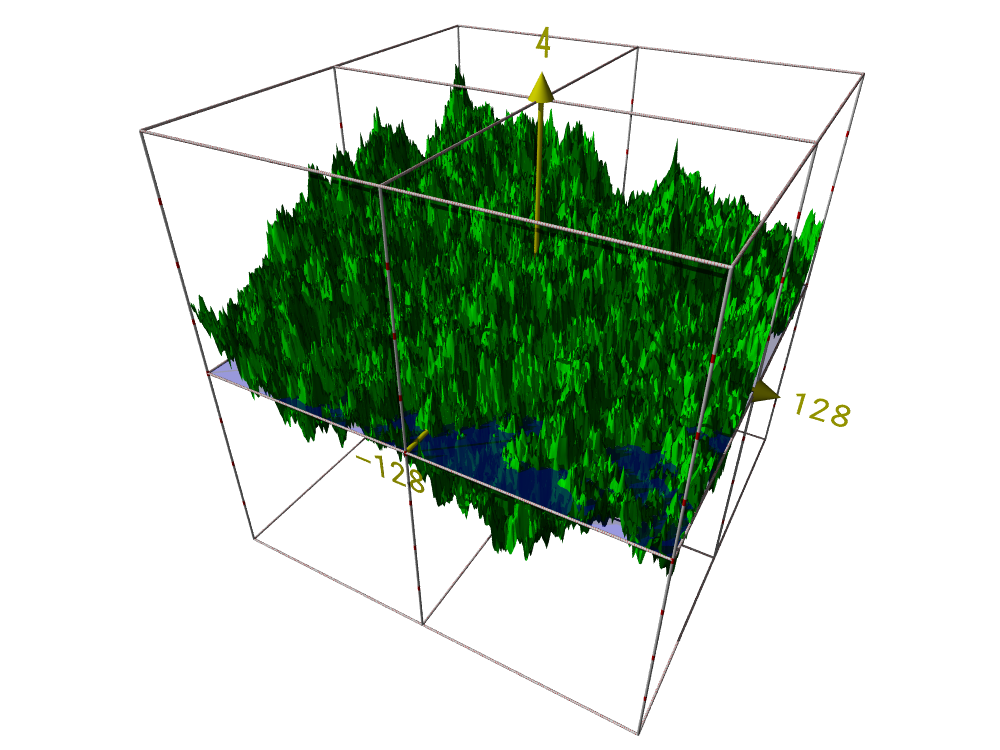
\includegraphics[width=\textwidth]{075.png}
    \caption{Randomness 0.75}
	\label{075}
  \end{minipage}
\end{figure}

\begin{figure}[H]
	\centering
	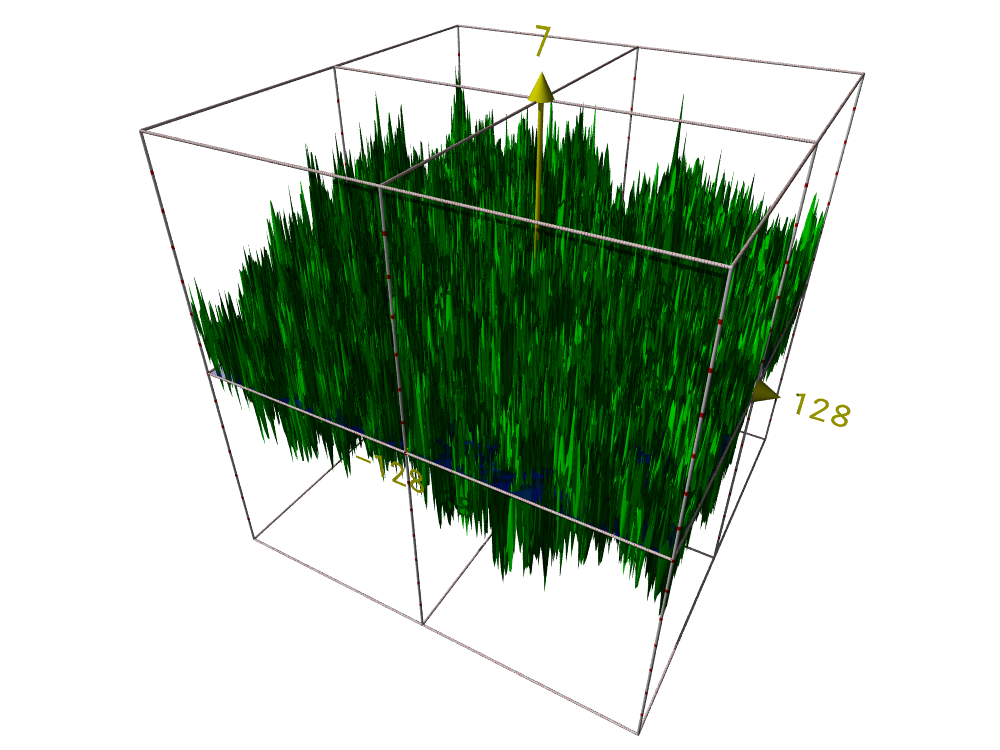
\includegraphics[width=0.5\textwidth]{100.png}
	\caption{Randomness 1.00}
	\label{100}
\end{figure}

\end{document}
